\documentclass[english,notitlepage]{article}  % defines the basic parameters of the document
\usepackage[T1]{fontenc} %for å bruke æøå
\usepackage[utf8]{inputenc}
\usepackage{graphicx} %for å inkludere grafikk
\usepackage{mathpazo}
\usepackage[norsk]{babel}
% Standard stuff
\usepackage{amsmath,graphicx,varioref,verbatim,amsfonts,geometry,gensymb, multirow}
% colors in text
\usepackage[usenames,dvipsnames,svgnames,table]{xcolor}
% Hyper refs
\usepackage[colorlinks=true,allcolors=black]{hyperref}

\usepackage{caption}
\usepackage{enumitem}
\usepackage{tikz}             % draw figures manually
\usepackage{subfigure}        % imports a lot of cool and useful figure commands
\usepackage{float}
\usepackage{circuitikz}
\usepackage{listings}
\lstset{basicstyle=\footnotesize\ttfamily,breaklines=true}

\usepackage{csquotes}
\usepackage[backend=biber,style=alphabetic,sorting=ynt]{biblatex} %Imports biblatex package
\addbibresource{referanser.bib}

\title{FYS3150\\Project 2}
\author{Brage A. Trefjord\\Sigurd Sønvisen Vargdal\\Frida Oleivsgard Sørensen\\Nils Enric Canut Taugbøl}


\begin{document}

\maketitle
\textit{GitHub repository:} \texttt{\url{https://github.com/NilsECT/FYS3150/tree/main/Project_2/Code}}


\section*{Problem 1:}

We use the dimensionless variable $\hat{x} = \frac{x}{L}$, which gives us
$\frac{d \hat{x}}{dx} = \frac{1}{L}$. Using this, we get:

\begin{align*}
    \frac{d}{dx} = \frac{d\hat{x}}{dx} \frac{d}{d\hat{x}} = \frac{1}{L} \frac{d}{d\hat{x}}
\end{align*}

And we can find the scaled differential equation:

\begin{align*}
    \gamma \frac{d^2 u(x)}{dx^2} &= -F u(x)
    \\
    \gamma \left( \frac{1}{L} \frac{d}{d\hat{x}} \right)^2 u(\hat{x}) &= -F u(\hat{x})
    \\
    \gamma \frac{1}{L^2} \frac{d^2 u(\hat{x})}{d \hat{x}^2} &= -F u(\hat{x})
    \\
    \frac{d^2 u(\hat{x})}{d \hat{x}^2} &= - \frac{F L^2}{\gamma} u(\hat{x})
    \\
    \frac{d^2 u(\hat{x})}{d \hat{x}^2} &= - \lambda u(\hat{x}) \; , \hspace*{20pt} \lambda \equiv \frac{F L^2}{\gamma}
\end{align*}


\section*{Problem 2}

Our tridiagonal $6 \times 6$ matrix is

\begin{equation*}
    A = \frac{1}{h^2} \begin{bmatrix}
        2 & -1 & 0 & 0 & 0 & 0 \\
        -1 & 2 & -1 & 0 & 0 & 0 \\
        0 & -1 & 2 & -1 & 0 & 0 \\
        0 & 0 & -1 & 2 & -1 & 0 \\
        0 & 0 & 0 & -1 & 2 & -1 \\
        0 & 0 & 0 & 0 & -1 & 2
    \end{bmatrix}
\end{equation*}

where $h = \frac{1}{N+1}$, and $N = 6$ is the dimension of our square matrix.

We solve the equation

\begin{equation*}
    A \vec{v} = \lambda \vec{v}
\end{equation*}

both analytically and using armadillo in \lstinline{C++}. Here $\lambda$ are the
eigenvalues, and $\vec{v}$ are the corresponding eigenvectors of $A$. See code
in repository. We find that the eigenvectors from armadillo are consistent with
those found analytically.


\section*{Problem 3}
\subsection*{a)}
We implement a method that identifies the indices of the largest off-diagonal element of a matrix. This method is in the GitHub repository, implemented as a class method \lstinline{find_k_l} in the \lstinline{Jacobi} class. This class is used for using Jacobi's rotation method for finding the eigenvalues and -vectors of $A$.

\subsection*{b)}
To test the \lstinline{find_k_l}-method, we implement a test function \lstinline{test_find_k_l} that asserts whether the method finds the correct indices for a test matrix. Our test matrix is

\begin{equation}
  A = \begin{bmatrix}1 & 0 & 0 & 0.5 \\
  0 & 1 & -0.7 & 0 \\
  0 & -0.7 & 1 & 0 \\
  0.5 & 0 & 0 & 1 \end{bmatrix}
\end{equation}

The code is in the repository.

\section*{Problem 4}
\subsection*{a)}
We write a code implementation of Jacobi's rotation algorithm by creating a class \lstinline{Jacobi} in \lstinline{C++}.

\subsection*{b)}
To test the solving method we write a program generating the test matrix. We use
Armadillos eigsym to test against. The code sorts the eigenvectors in order of
rising eigenvalue. It then checks if the two matrices are equal, within a tolerance
of $1e-7$. The code prints a statement telling us if the two matrices are equal.

\section*{Problem 5}
\subsection*{a)}
The code for this problem is in the repository.
We have an $N \times N$ tridiagonal matrix.

\begin{figure}[H]
    \centering
    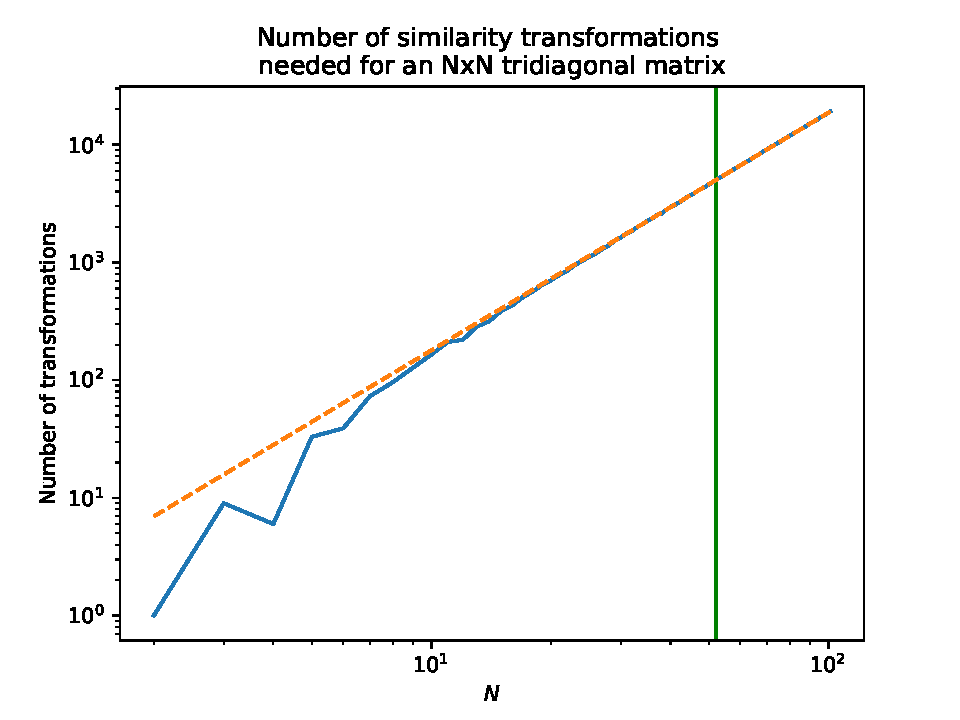
\includegraphics[width=0.8\linewidth]{../Code/Problem_5_plot.pdf}
    \caption{Logarithmic plot of the number of transformations needed to compute the eigenvalues for an $N \times N$ tridiagonal matrix with a tolerance of 1e-10. We see that the curve is linear after a certain $N$, and therefore construct a linear regression for the curve after this $N$-value. The green line shows where we started our linear regression of the curve.}
    \label{fig:5plot}
\end{figure}

In \hyperref[fig:5plot]{Figure \ref*{fig:5plot}} we have plotted the number of
transformations used by the algorithm when we calculated the eigenvectors of
tridiagonal $N \times N$ matrices. The plot is logarithmic, and after a certain
$N$ the curve looks linear. Since it is linear we have made a linear regression
for the curve for high values of $N$, and plotted this line together with our
curve. We get that the linear regression has a slope of $2.02$. Since the plot
is logarithmic, this tells us that the number of transformations is
approximately of order $O(N^2)$.


\subsection*{b)}
During our transformations in the Jacobi method, we mess around with all the
other values in the matrix, not just the ones we want to change. When trying to
zero out one element, another element goes from zero to something. After enough
transformations this still converges to a diagonal matrix, where all other
elements are approximately zero. In the process of the transformations however,
the zero-values of our tridiagonal matrix becomes non-zero. Our matrix can
therefore, after a certain amount of transformations, be seen as a dense matrix.
Since our tridiagonal matrix becomes dense in the process of the algorithm, we
assume that using this algorithm on a dense matrix would require an
approximately equal amount of transformations as the tridiagonal case.

\section*{Problem 6}
\subsection*{a)}
We use a discretization with $n=10$ steps, and plot the three eigenvectors $\vec{v}$ corresponding to the lowest three eigenvalues. Our solver yields the discretized eigenvectors $\vec{v} = [ v_1, v_2, ..., v_{N} ]$ where $N=n-1$ and $n$ is the number of steps in the discretization. As this vector only contains the inner points of the solution, we include the boundary points $v_0 = 0$ and $v_n = 0$ by adding these manually before plotting.

See \hyperref[fig:6aplot]{figure \ref*{fig:6aplot}} for the plot. The code for this is in the repository. We see that for the eigenvector $\vec{v}_1$, the analytical and the numerical differ by a factor of $-1$ (meaning the signs are opposite). We assume this may be due to \lstinline{Armadillo}'s \lstinline{eig_sym}-function

\begin{figure}[H]
    \centering
    \includegraphics[width=0.8\linewidth]{../Code/Problem_6_a_plot.pdf}
    \caption{Plot of the eigenvectors $\vec{v}$ corresponding to the 3 lowest eigenvalues, including the boundary conditions 0 at the start and the beginning. A discretization of $n=10$ steps is used.}
    \label{fig:6aplot}
\end{figure}

\subsection*{b)}

We do the same, this time using $n=100$ steps. See \hyperref[fig:6bplot]{figure \ref*{fig:6bplot}} for the plot.

\begin{figure}[H]
    \centering
    \includegraphics[width=0.8\linewidth]{../Code/Problem_6_b_plot.pdf}
    \caption{Plot of the eigenvectors $\vec{v}$ corresponding to the 3 lowest eigenvalues, including the boundary conditions 0 at the start and the beginning. A discretization of $n=100$ steps is used.}
    \label{fig:6bplot}
\end{figure}

\end{document}
